
\section{Tassu ennen vanhaan}
\textit{Tassu on ilmestynyt säännöllisen epäsäännöllisesti lippukunnan perustamisvuodesta 1986
lähtien. Tällä palstalla muistellaan menneitä ja julkaistaan valittuja paloja takavuosien
lehdistä.}

% \textit{Päätoimittaja sai paketin, jossa on vuosikymmeniä Tassun painoksia ja
% yrittää digitalisoida ne lähiaikoina!}

\vspace*{0.32cm}
\noindent Tällä kertaa mennään ajassa 30 vuotta taaksepäin, ja Eddien muistoa
kunnioittaen luetaan tervehdys vuodelta 1995:

\newtcolorbox{StickyNote}[1][]{%
    enhanced,
    before skip=2mm,after skip=2mm, 
    width=\textwidth, boxrule=0.4mm, % width of the sticky note
    colback=white, colframe=kuru, % Colors
    attach boxed title to top right={xshift=0cm,yshift*=0mm-\tcboxedtitleheight},
    varwidth boxed title*=-3cm,
    % The titlebox:
    boxed title style={frame code={%
        \path[left color=kuru,right color=kuru,
        middle color=kuru]
        ([xshift=-0mm]frame.north west) -- ([xshift=0mm]frame.north east)
        [rounded corners=0mm]-- ([xshift=0mm,yshift=0mm]frame.north east)
        -- (frame.south east) -- (frame.south west)
        -- ([xshift=0mm,yshift=0mm]frame.north west)
        [sharp corners]-- cycle;
        },interior engine=empty,
    },
    sharp corners,rounded corners=southeast,arc is angular,arc=3mm,
    % The "folded paper" in the bottom right corner:
    underlay={%
        \path[fill=kuru!80!black] ([yshift=3mm]interior.south east)--++(-0.4,-0.1)--++(0.1,-0.2);
        \path[draw=kuru,shorten <=-0.05mm,shorten >=-0.05mm,color=kuru] ([yshift=3mm]interior.south east)--++(-0.4,-0.1)--++(0.1,-0.2);
        },
    % drop fuzzy shadow, % Shadow
    % fonttitle=\bfseries, 
    title={#1}
}

\vspace*{1.28cm}
\begin{StickyNote}[Julkaistu alunperin Tassussa 2/1995]
	\monofont

	% \begin{center}
	% 	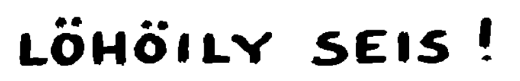
\includegraphics[width=6cm]{assets/löhöilyseis1}
	% \end{center}

	\begin{center}
		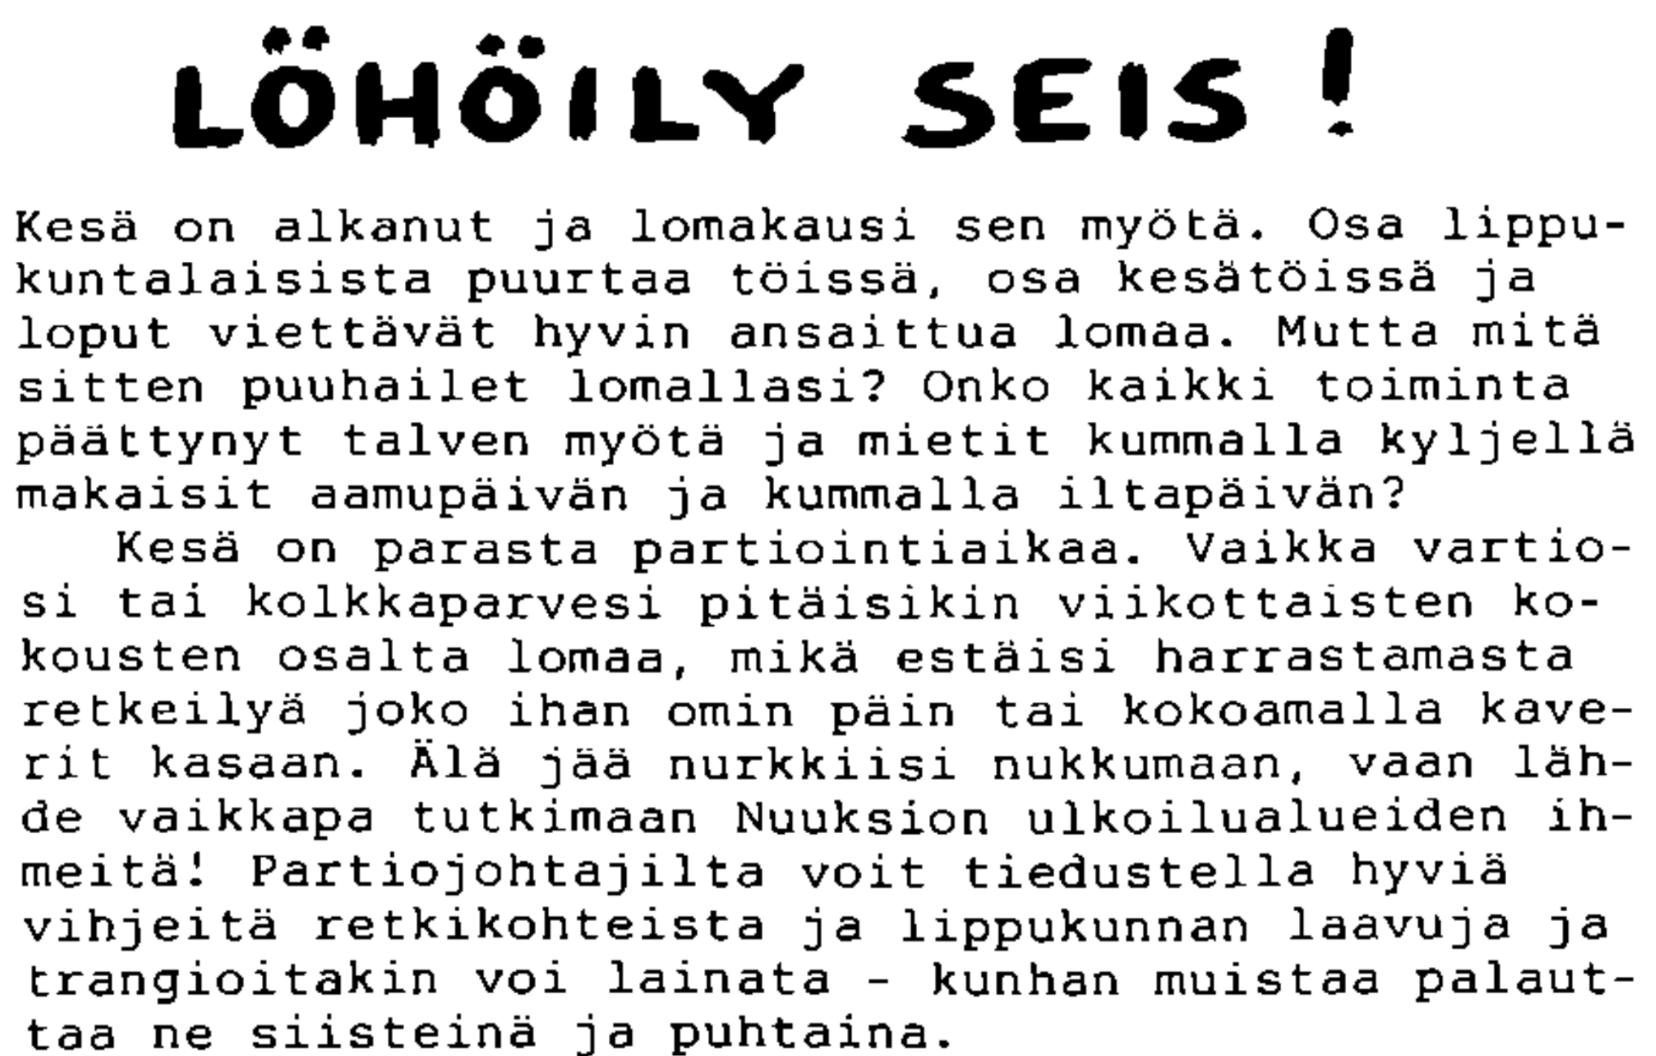
\includegraphics[width=1\textwidth]{assets/löhöilyseis3}
	\end{center}

% 	Kesä on alkanut ja lomakausi sen myötä. Osa lippu-kuntalaisista puurtaa
% 	töissä, osa kesätöissä ja loput viettävät hyvin ansaittua lomaa. Mutta
% 	mitä sitten puuhailet lomallasi? Onko kaikki toiminta päättynyt talven
% 	myötä ja mietit kummalla kyljellä makaisit aamupäivän ja kummalla
% 	iltapäivän?

% 	\smallskip
% 	\hspace{0.32cm}
% 	Kesä on parasta partiointiaikaa. Vaikka vartio-si tai kolkkaparvesi
% 	pitäisikin viikottaisten ko-kousten osalta lomaa, mikä estäisi
% 	harrastamasta retkeilyä joko ihan omin päin tai kokoamalla kave-rit
% 	kasaan. Älä jää nurkkiisi nukkumaan, vaan läh-de vaikkapa tutkimaan
% 	Nuuksion ulkoilualueiden ih-meitä! Partiojohtajilta voit tiedustella
% 	hyviä vihjeitä retkikohteista ja lippukunnan laavuja ja trangioitakin
% 	voi lainata kunhan muistaa palaut-taa ne siisteinä ja puhtaina.

	\vspace*{0.08cm}
	{\hspace{0.16cm}\Large\ldots}
	\vspace*{0.32cm}

\end{StickyNote}

\clearpage

\vspace*{1.28cm}
\begin{StickyNote}[Julkaistu alunperin Tassussa 2/1995]
	\monofont

	{\hspace{0.16cm}\Large\ldots}
	\vspace*{0.16cm}

	\begin{center}
		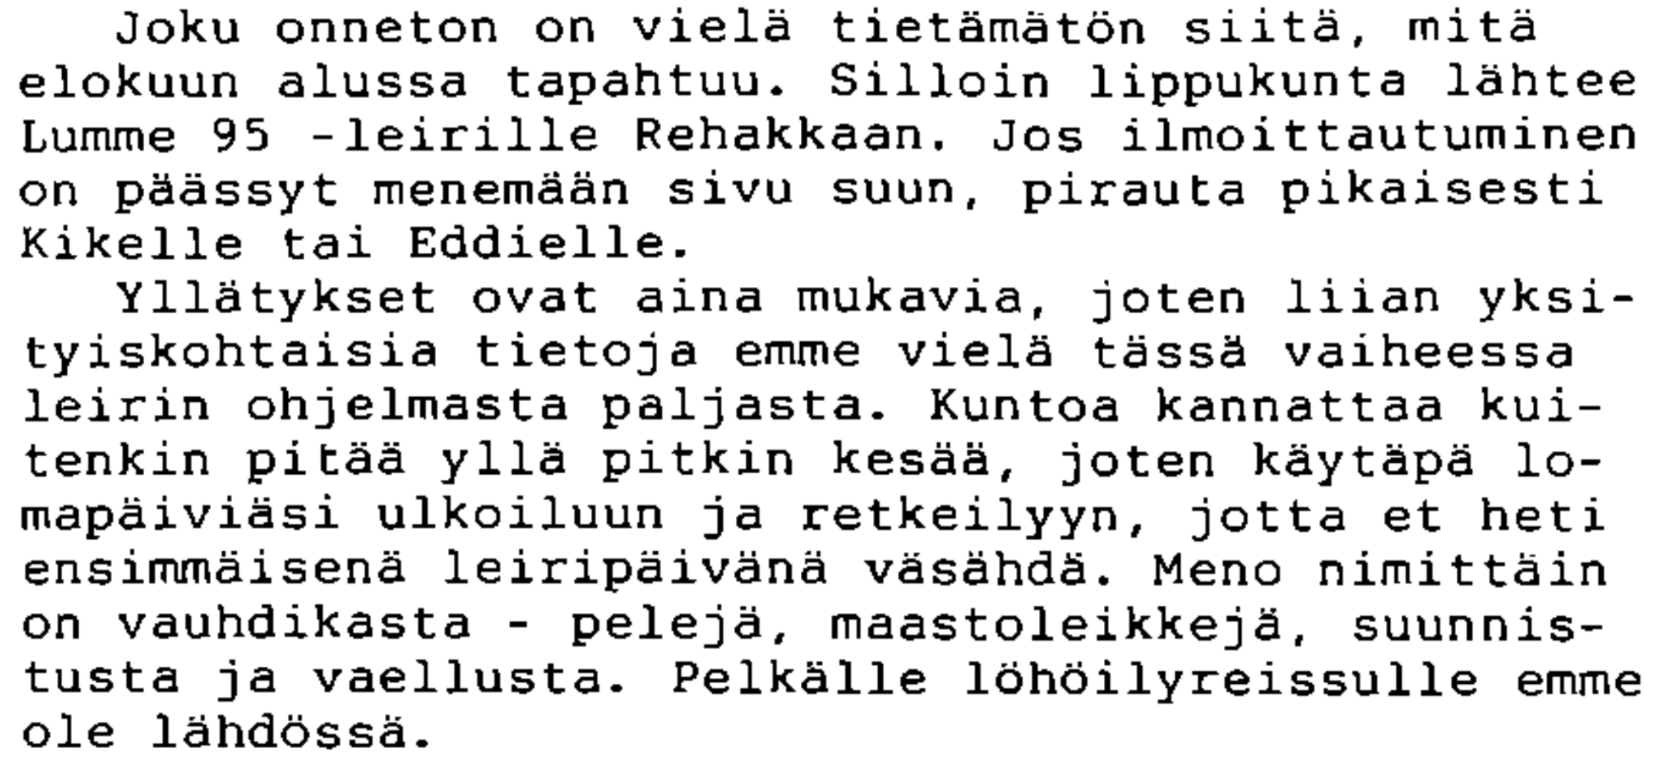
\includegraphics[width=1\textwidth]{assets/löhöilyseis4}
		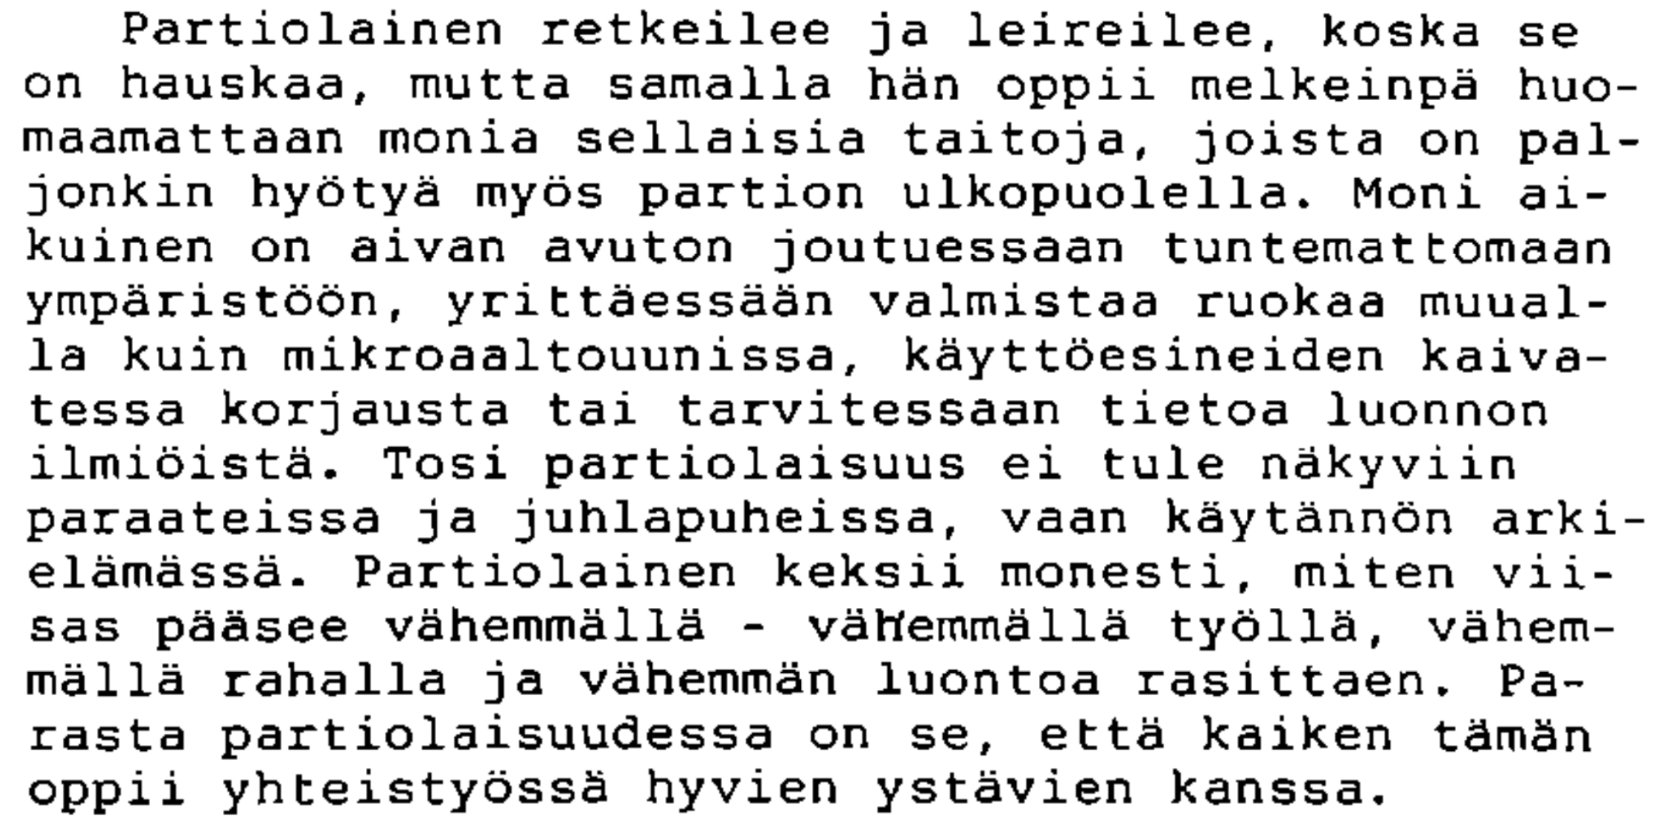
\includegraphics[width=1\textwidth]{assets/löhöilyseis5}
	\end{center}

	% \smallskip
	% \hspace{0.32cm}
	% Joku onneton on vielä tietämätön siitä, mitä elokuun alussa tapahtuu.
	% Silloin lippukunta lähtee Lumme 95-leirille Rehakkaan. Jos
	% ilmoittautuminen on päässyt menemään sivu suun, pirauta pikaisesti
	% Kikelle tai Eddielle.

	% \smallskip
	% \hspace{0.32cm}
	% Yllätykset ovat aina mukavia, joten liian yksi-tyiskohtaisia tietoja
	% emme vielä tässä vaiheessa leirin ohjelmasta paljasta. Kuntoa kannattaa
	% kui-tenkin pitää yllä pitkin kesää, joten käytäpä lo-mapäiviäsi
	% ulkoiluun ja retkeilyyn, jotta et heti ensimmäisenä leiripäivänä
	% väsähdä. Meno nimittäin on vauhdikasta pelejä, maastoleikkejä,
	% suunnis-tusta ja vaellusta. Pelkälle löhöilyreissulle emme ole
	% lähdössä.

	% \smallskip
	% \hspace{0.32cm}
	% Partiolainen retkeilee ja leireilee, koska se on hauskaa, mutta samalla
	% hän oppii melkeinpä huo-maamattaan monia sellaisia taitoja, joista on
	% pal-jonkin hyötyä myös partion ulkopuolella. Moni ai-kuinen on aivan
	% avuton joutuessaan tuntemattomaan ympäristöön, yrittäessään valmistaa
	% ruokaa muual-la kuin mikroaaltouunissa, käyttöesineiden kaiva-tessa
	% korjausta tai tarvitessaan tietoa luonnon ilmiöistä. Tosi partiolaisuus
	% ei tule näkyviin paraateissa ja juhlapuheissa, vaan käytännön
	% arki-elämässä. Partiolainen keksii monesti, miten viisas pääsee
	% vähemmällä - vähemmällä työllä, vähemmällä rahalla ja vähemmän luontoa
	% rasittaen. Parasta partiolaisuudessa on se, että kaiken tämän oppii
	% yhteistyössä hyvien ystävien kanssa.

	\noindent\null\hfill
\includegraphics[width=4cm]{assets/löhöilyseis2}

\end{StickyNote}
